\section{Vehicle Emissions}
\label{sec:Results_Emissions}

The environmental impact of the control strategies is evaluated by focusing on the average \ac{co2} and \ac{nox} mass per kilometre, as detailed in Table~\vref{tab:Emissions}. The results, visualized in Figures~\vref{fig:Emis_692} through \vref{fig:Emis_3462}, are discussed separately for the HBEFA4 and PHEMlight5 models, as their different sensitivities to transient vehicle dynamics yield distinct outcomes.

\paragraph{Low to Intermediate Demand ($69$--$692~\unit{\veh\per\hour}$).}
In the low-to-intermediate demand range, both controllers generally yield emission benefits. Under the HBEFA4 model, these benefits become more consistent as demand increases. For instance, at a traffic demand of $692~\unit{\veh\per\hour}$, where the baseline emission is $148.06~\unit{\gram\per\kilo\metre}$ of \ac{co2}, the improvements at full \ac{mpr} are significant. The \ac{eco-glosa} controller reduces \ac{co2} emissions to $141.17~\unit{\gram\per\kilo\metre}$ (a $4.7\%$ reduction), while the \ac{flow-glosa} algorithm achieves a greater benefit, reducing emissions to $139.50~\unit{\gram\per\kilo\metre}$ (a $5.8\%$ reduction). As illustrated in Figure~\vref{fig:Emis_692_HBEFA4}, increasing the \ac{mpr} for both strategies leads to a steady decrease in both \ac{co2} and \ac{nox} emissions.
\mynewline
The PHEMlight5 model presents a different perspective, with benefits that are strongly dependent on the \ac{mpr} (Figure~\vref{fig:Emis_692_PHEM}). At $692~\unit{\veh\per\hour}$, the \ac{flow-glosa} algorithm achieves a consistent, modest \ac{co2} reduction across all penetration rates. In contrast, \ac{eco-glosa} provides substantial \ac{co2} reductions at high \acp{mpr}, achieving a benefit of nearly $6\%$ at $100\%$ \ac{mpr}, where emissions fall from a baseline of $157.36~\unit{\gram\per\kilo\metre}$ to $147.94~\unit{\gram\per\kilo\metre}$. A significant finding from PHEMlight5 remains the potential trade-off between \ac{co2} and \ac{nox} emissions. While \ac{co2} emissions improve, \ac{nox} emissions from \ac{eco-glosa} initially increase, rising from a baseline of $0.0551~\unit{\gram\per\kilo\metre}$ to $0.0561~\unit{\gram\per\kilo\metre}$ at $30\%$ \ac{mpr}, before falling below the baseline at higher penetration rates.

\begin{figure}[htbp]
  \centering
  \begin{subfigure}[b]{0.98\textwidth}
    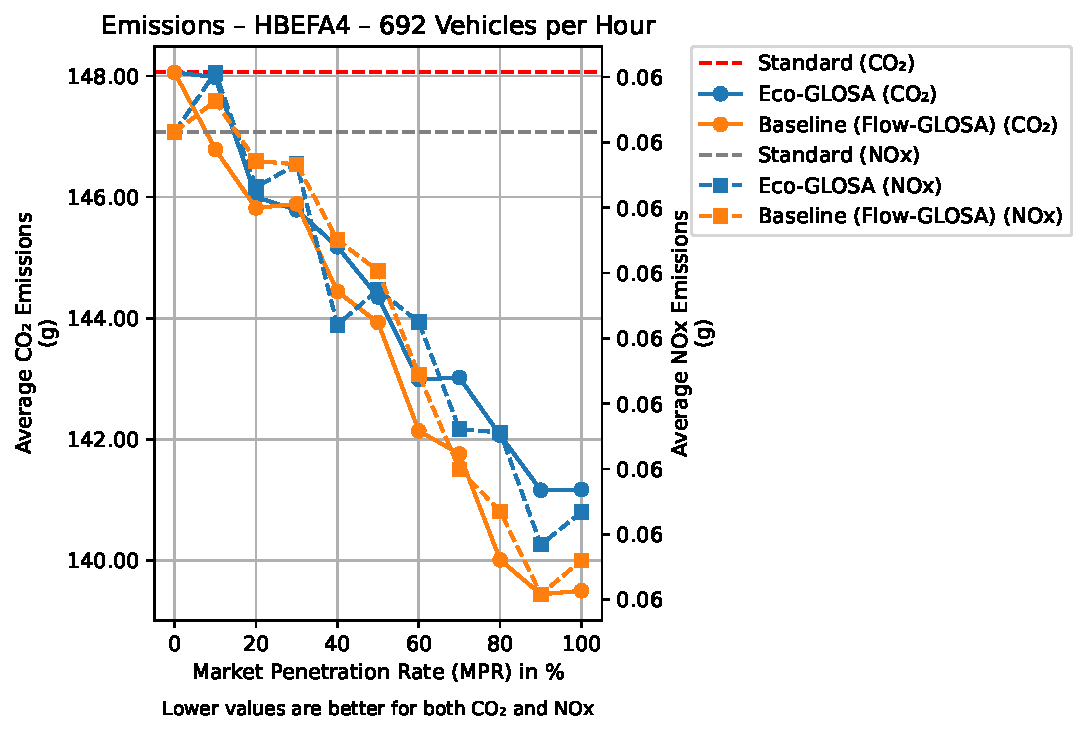
\includegraphics[width=\textwidth]{data/img/Emissions/Emissions_HBEFA4_Cars692.pdf}
    \caption{HBEFA4 at $692\,\mathrm{veh/h}$.}
    \label{fig:Emis_692_HBEFA4}
  \end{subfigure}
  \begin{subfigure}[b]{0.98\textwidth}
    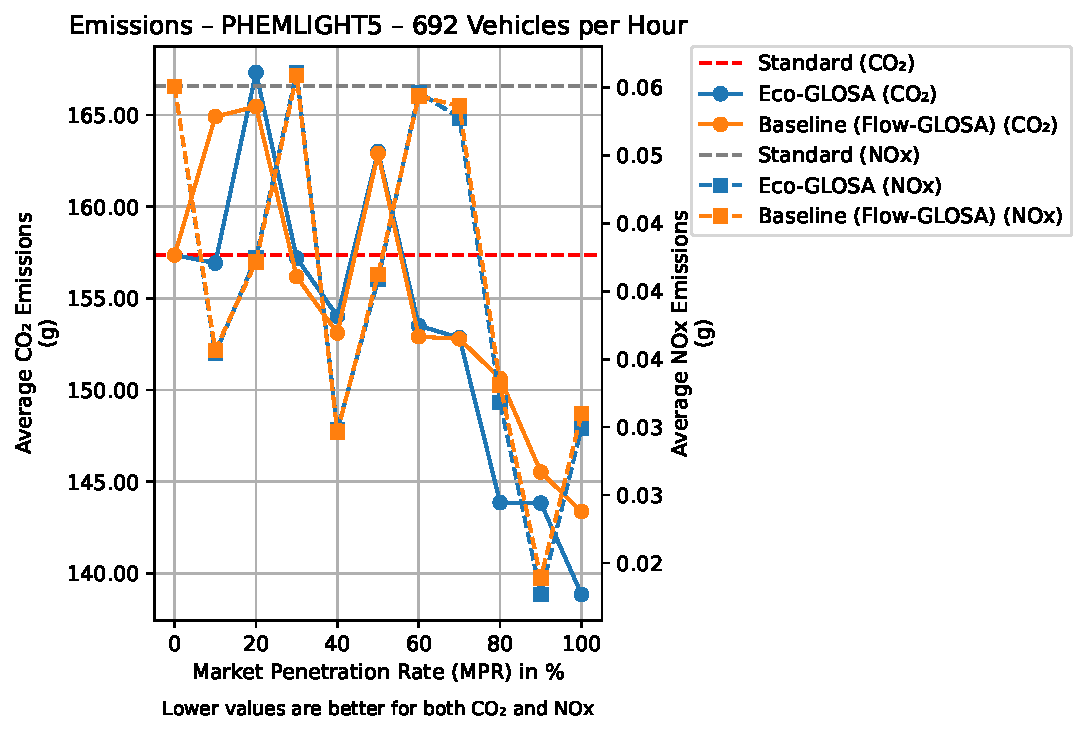
\includegraphics[width=\textwidth]{data/img/Emissions/Emissions_PHEMLIGHT5_Cars692.pdf}
    \caption{PHEMlight5 at $692\,\mathrm{veh/h}$.}
    \label{fig:Emis_692_PHEM}
  \end{subfigure}
  \caption[\ac{co2} and \ac{nox} emissions vs. \ac{mpr} at $692~\unit{\veh\per\hour}$]{\ac{co2} and \ac{nox} emissions versus \ac{mpr} at a low demand of $692~\unit{\veh\per\hour}$.}
\label{fig:Emis_692}
\end{figure}

\paragraph{Emerging Congestion ($1385$--$2077~\unit{\veh\per\hour}$).}
As traffic demand enters the range of emerging congestion, the \ac{eco-glosa} controller realizes measurable emission savings with the HBEFA4 model. At a demand of $1385~\unit{\veh\per\hour}$, the algorithm lowers \ac{co2} emissions from the Standard of $149.86~\unit{\gram\per\kilo\metre}$ to $143.37~\unit{\gram\per\kilo\metre}$ at $80\%$ \ac{mpr}, a reduction of $4.3\%$. This is accompanied by a $5.3\%$ decrease in \ac{nox} emissions. At $2077~\unit{\veh\per\hour}$, full penetration of \ac{eco-glosa} reduces \ac{co2} by $6.2\%$ and \ac{nox} by $7.1\%$. The throughput-oriented \ac{flow-glosa} controller performs even better under these conditions. At the same $2077~\unit{\veh\per\hour}$ demand, it reduces \ac{co2} emissions by a more substantial $8.5\%$ (to $139.96~\unit{\gram\per\kilo\metre}$) and achieves a comparable \ac{nox} reduction of $7.5\%$.
\mynewline
The PHEMlight5 model demonstrates the same qualitative trend, although the magnitude of the savings is attenuated. In the $2077~\unit{\veh\per\hour}$ scenario, \ac{eco-glosa} decreases \ac{co2} emissions from a baseline of $162.83~\unit{\gram\per\kilo\metre}$ to $154.63~\unit{\gram\per\kilo\metre}$ at $100\%$ \ac{mpr}, a modest reduction of $5.0\%$. Here too, the \ac{flow-glosa} strategy demonstrates a superior outcome, reducing \ac{co2} emissions by $6.6\%$ to $152.12~\unit{\gram\per\kilo\metre}$ and delivering a more significant \ac{nox} reduction of $8.5\%$. A comparison of the results in Figures~\vref{fig:Emis_2077_HBEFA4} and \vref{fig:Emis_2077_PHEM} corroborates this difference, suggesting the higher transient fidelity of the PHEMlight5 model provides a more conservative estimate of the achievable benefits.

\begin{figure}[htbp]
  \centering
  \begin{subfigure}[b]{0.98\textwidth}
    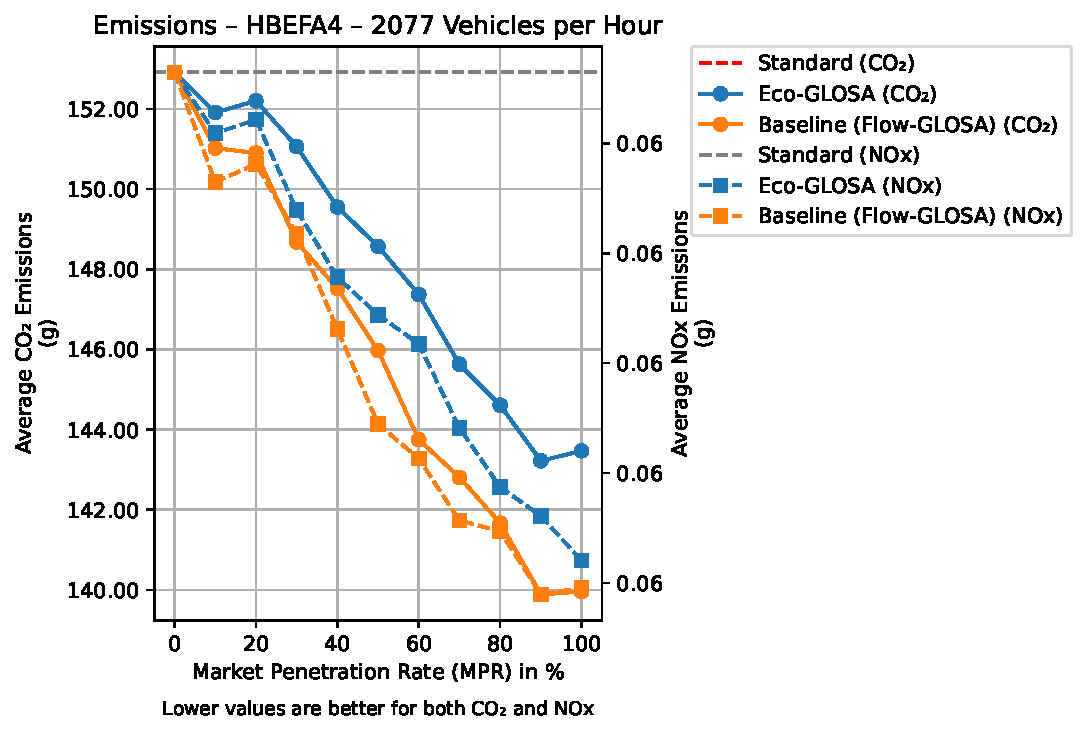
\includegraphics[width=\textwidth]{data/img/Emissions/Emissions_HBEFA4_Cars2077.pdf}
    \caption{HBEFA4 at $2077\,\mathrm{veh/h}$.}
    \label{fig:Emis_2077_HBEFA4}
  \end{subfigure}
  \begin{subfigure}[b]{0.98\textwidth}
    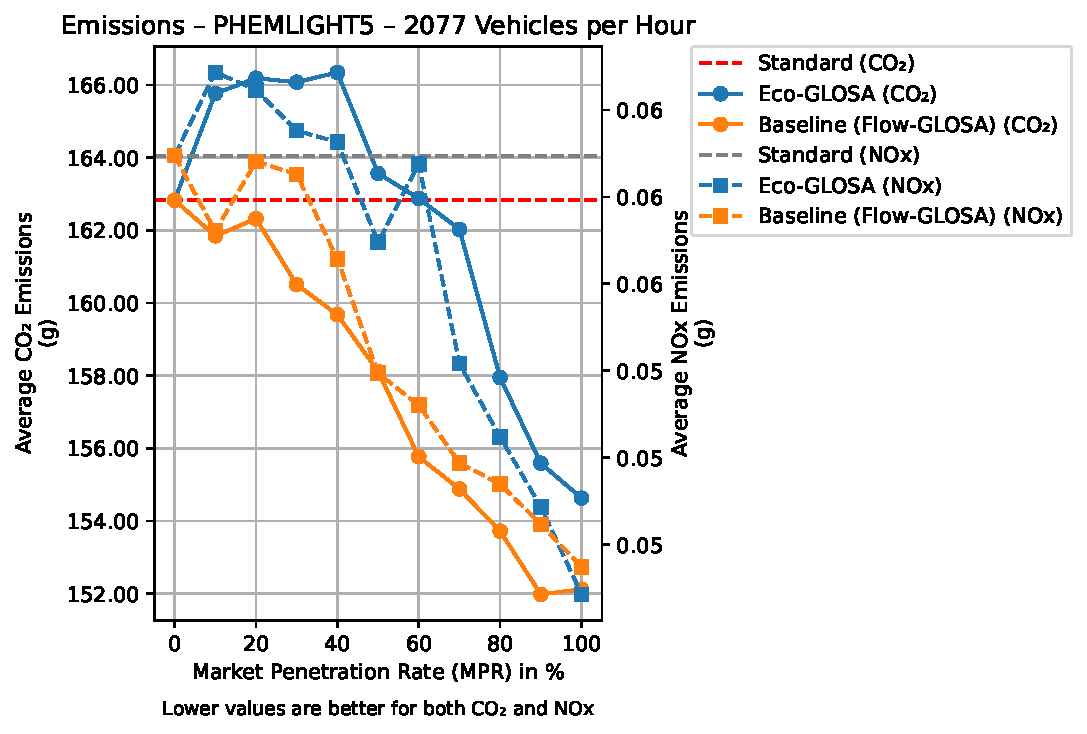
\includegraphics[width=\textwidth]{data/img/Emissions/Emissions_PHEMLIGHT5_Cars2077.pdf}
    \caption{PHEMlight5 at $2077\,\mathrm{veh/h}$.}
    \label{fig:Emis_2077_PHEM}
  \end{subfigure}
  \caption[\ac{co2} and \ac{nox} emissions vs. \ac{mpr} at $2077~\unit{\veh\per\hour}$]{\ac{co2} and \ac{nox} emissions versus \ac{mpr} under emerging congestion at $2077~\unit{\veh\per\hour}$.}
  \label{fig:Emis_2077}
\end{figure}

\paragraph{High Demand ($2769~\unit{\veh\per\hour}$).}
This demand level represents a critical turning point where the \ac{eco-glosa} controller's performance begins to decline. Instead of improvements, this leads to enormous emission spikes. Under the HBEFA4 model, the most severe outlier occurs at $60\%$ \ac{mpr}, where \ac{co2} emissions jump to $419.09~\unit{\gram\per\kilo\metre}$ and \ac{nox} emissions to $0.1730~\unit{\gram\per\kilo\metre}$, representing increases of $164\%$ and $159\%$ over the Standard, respectively. As seen in Figure~\vref{fig:Emis_2769_HBEFA4}, these excursions correspond to severe stop-and-go waves. In contrast, the \ac{flow-glosa} controller's emissions remain bounded and consistently below the Standard, showcasing its superior stability.
\mynewline
Under the PHEMlight5 model, the traffic jam is fully established at this demand, leading to poor performance for the \ac{eco-glosa} controller across all penetration rates. Its \ac{co2} emissions rise from the Standard of $168.29~\unit{\gram\per\kilo\metre}$ to a peak of $347.73~\unit{\gram\per\kilo\metre}$ at $70\%$ \ac{mpr}. Unlike the erratic spikes in the HBEFA4 model, PHEMlight5 predicts a more uniformly high emission profile for \ac{eco-glosa} in this congested state. This disparity stems from the model’s detailed transient engine maps, which impose a steep penalty on the inefficient, low-speed, high-load conditions that characterize a persistent traffic jam.

\begin{figure}[htbp]
  \centering
  \begin{subfigure}[b]{0.98\textwidth}
    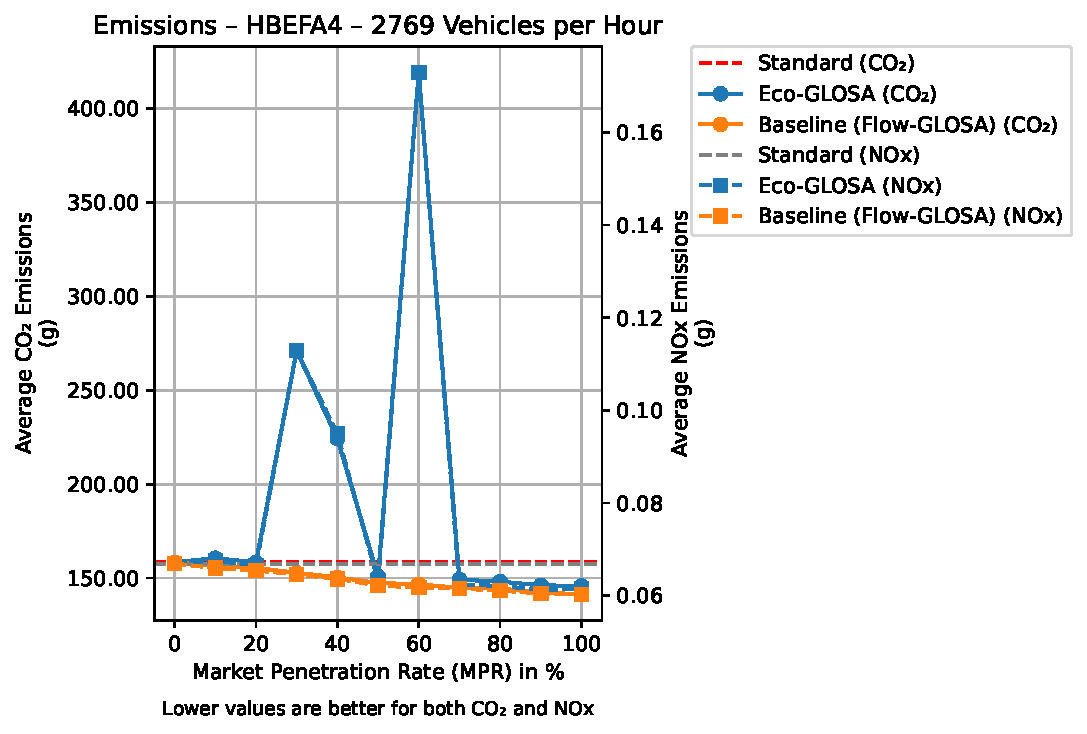
\includegraphics[width=\textwidth]{data/img/Emissions/Emissions_HBEFA4_Cars2769.pdf}
    \caption{HBEFA4 at $2769\,\mathrm{veh/h}$.}
    \label{fig:Emis_2769_HBEFA4}
  \end{subfigure}
  \begin{subfigure}[b]{0.98\textwidth}
    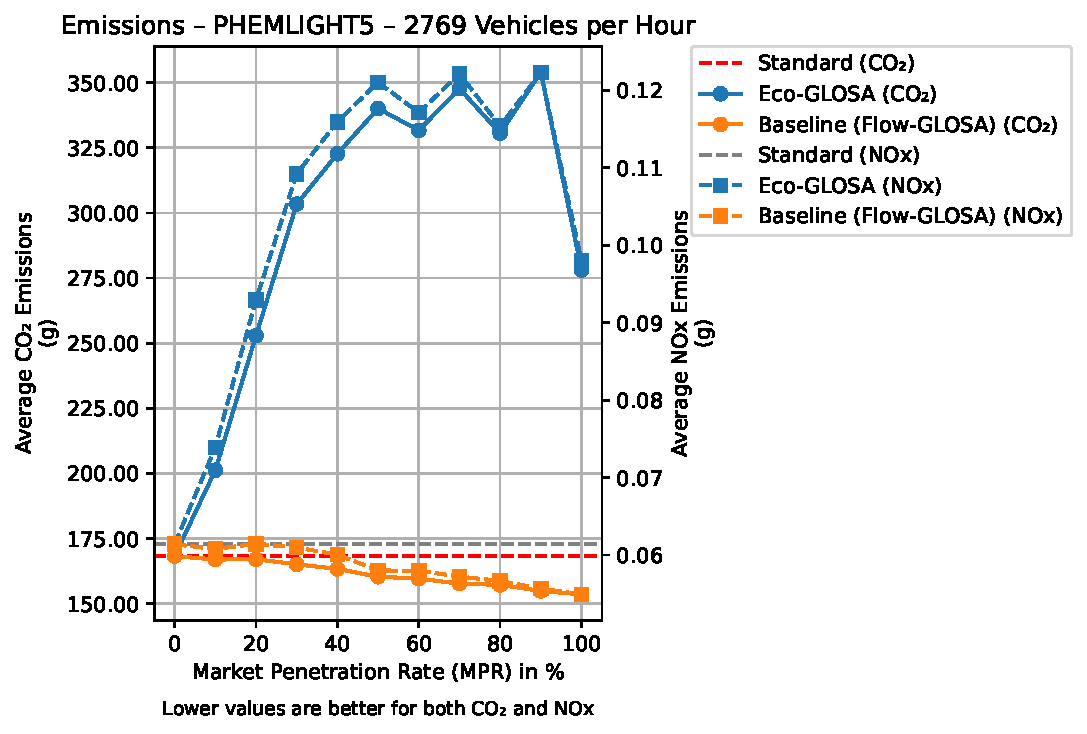
\includegraphics[width=\textwidth]{data/img/Emissions/Emissions_PHEMLIGHT5_Cars2769.pdf}
    \caption{PHEMlight5 at $2769\,\mathrm{veh/h}$.}
    \label{fig:Emis_2769_PHEM}
  \end{subfigure}
  \caption[\ac{co2} and \ac{nox} emissions vs. \ac{mpr} at $2769~\unit{\veh\per\hour}$]{\ac{co2} and \ac{nox} emissions versus \ac{mpr} at a high demand of $2769~\unit{\veh\per\hour}$, showing significant performance degradation for \ac{eco-glosa}.}
  \label{fig:Emis_2769}
\end{figure}

\paragraph{Saturated Regime ($3462~\unit{\veh\per\hour}$).}
The contrasting relationship between the two control methods is most striking in the fully saturated scenario (Figure~\ref{fig:Emis_3462}). Under the HBEFA4 model, the \ac{eco-glosa} controller consistently degrades performance as penetration increases, its \ac{co2} emissions soaring from the already high Standard of $426.68~\unit{\gram\per\kilo\metre}$ to a peak of $603.19~\unit{\gram\per\kilo\metre}$ at $100\%$ \ac{mpr}. Conversely, the \ac{flow-glosa} controller prevents the system from remaining in a gridlocked state. Under HBEFA4, its application causes \ac{co2} emissions to plummet from $426.68~\unit{\gram\per\kilo\metre}$ to just $142.78~\unit{\gram\per\kilo\metre}$ at $100\%$ \ac{mpr}, a reduction of over $66\%$. By preventing a severe jam, emissions settle on a low plateau as vehicles traverse the corridor at a stable free-flow speed. This advantage is even more pronounced with the PHEMlight5 model. At full penetration, \ac{eco-glosa} still produces $412.78~\unit{\gram\per\kilo\metre}$ of \ac{co2}, whereas \ac{flow-glosa} emits only $155.50~\unit{\gram\per\kilo\metre}$. These findings reveal that a control law aimed at maximising throughput can noticeably outperform an explicitly eco-oriented variant in heavily congested traffic.

\begin{figure}[htbp]
  \centering
  \begin{subfigure}[b]{0.98\textwidth}
    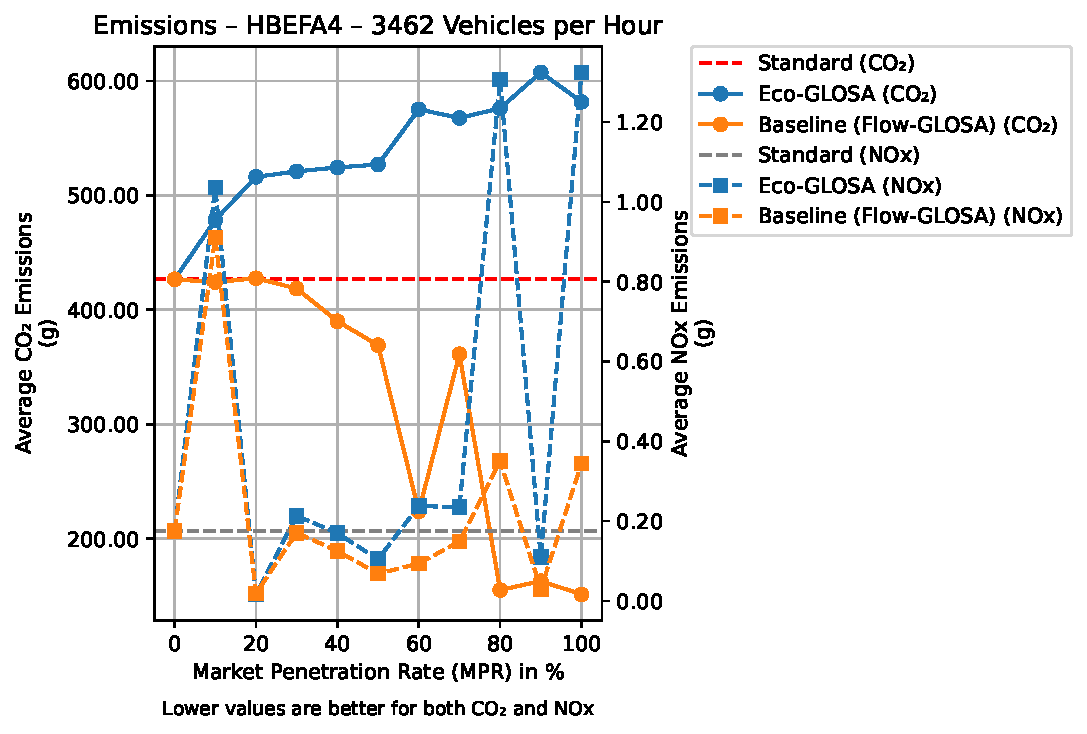
\includegraphics[width=\textwidth]{data/img/Emissions/Emissions_HBEFA4_Cars3462.pdf}
    \caption{HBEFA4 at $3462\,\mathrm{veh/h}$.}
    \label{fig:Emis_3462_HBEFA4}
  \end{subfigure}
  \begin{subfigure}[b]{0.98\textwidth}
    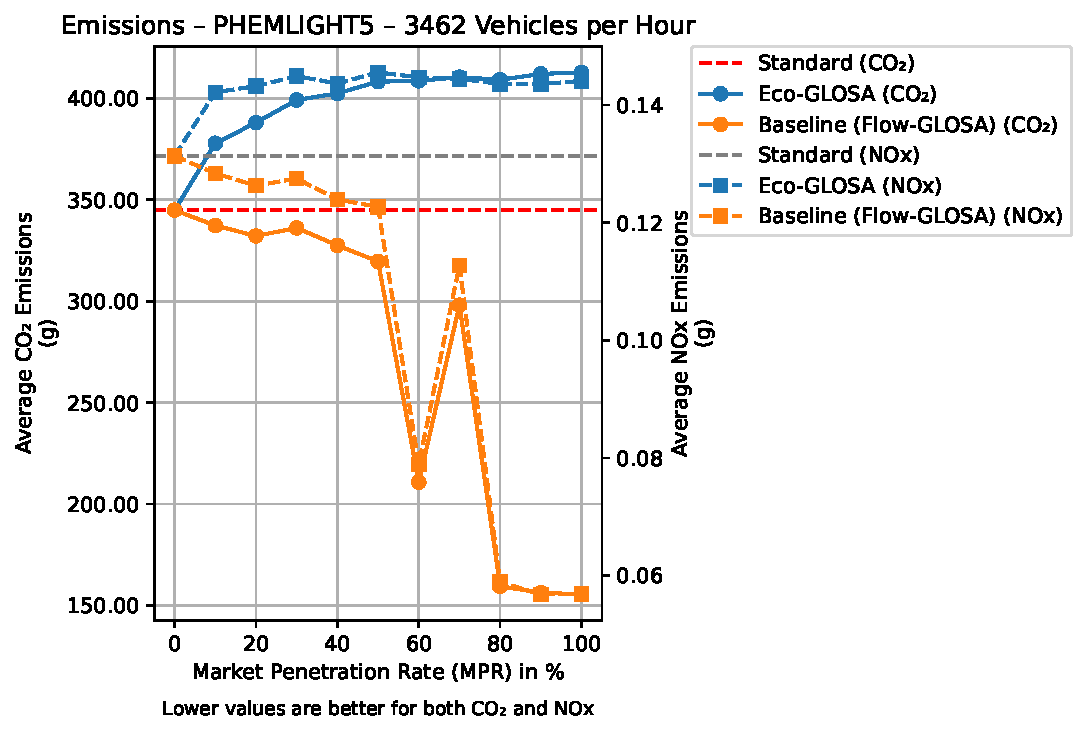
\includegraphics[width=\textwidth]{data/img/Emissions/Emissions_PHEMLIGHT5_Cars3462.pdf}
    \caption{PHEMlight5 at $3462\,\mathrm{veh/h}$.}
    \label{fig:Emis_3462_PHEM}
  \end{subfigure}
  \caption[\ac{co2} and \ac{nox} emissions vs. \ac{mpr} at $3462~\unit{\veh\per\hour}$]{\ac{co2} and \ac{nox} emissions versus \ac{mpr} in the fully saturated regime ($3462~\unit{\veh\per\hour}$), highlighting the superior performance of \ac{flow-glosa}.}
  \label{fig:Emis_3462}
\end{figure}

\paragraph{Implications.}
Comparing the HBEFA4 and PHEMlight5 models reveals two key differences. First, they provide different estimates of the absolute benefits of \ac{flow-glosa} in saturation. For the $3462~\unit{\veh\per\hour}$ scenario, HBEFA4 predicts a \ac{co2} reduction of approximately $66\%$, while PHEMlight5 estimates a still substantial $55\%$ reduction. This discrepancy arises because the Standard emission value for HBEFA4 ($426.68~\unit{\gram\per\kilo\metre}$) is significantly higher than that of PHEMlight5 ($344.88~\unit{\gram\per\kilo\metre}$), suggesting its static factors may inadequately capture engine behaviour during prolonged idling. Second, the models diverge in their sensitivity to \ac{eco-glosa}'s performance degradation. At $2769~\unit{\veh\per\hour}$, the PHEMlight5 model shows that \ac{eco-glosa} becomes counterproductive almost immediately, whereas the HBEFA4 results are more volatile, showing severe but inconsistent emission spikes.
\mynewline
A granular analysis separating equipped from non-equipped vehicles reveals the direct impact on the user. Under \ac{eco-glosa}, equipped vehicles consistently exhibit lower \ac{co2} emissions than their unequipped counterparts. For instance, under the PHEMlight5 model at a demand of $1385~\unit{\veh\per\hour}$ and $90\%$ \ac{mpr}, equipped vehicles emit $151.21~\unit{\gram\per\kilo\metre}$ of \ac{co2}, which is $5.5\%$ less than the $160.01~\unit{\gram\per\kilo\metre}$ from unequipped vehicles in the same traffic stream. This demonstrates that the controller successfully optimises the individual vehicle's trajectory for fuel efficiency. However, under \ac{flow-glosa}, the opposite can be true, as equipped vehicles may be required to accelerate more aggressively to maintain flow for the benefit of the overall system. A clear example occurs with the HBEFA4 model at $69~\unit{\veh\per\hour}$ and $10\%~\ac{mpr}$, where equipped \ac{flow-glosa} vehicles emit $153.44~\unit{\gram\per\kilo\metre}$, slightly more than the $143.36~\unit{\gram\per\kilo\metre}$ from their unequipped peers. This underscores a key paradox: the high physical fidelity of PHEMlight5 accurately penalises the energy cost of transient manoeuvres. \ac{eco-glosa}, in its strict pursuit of minimising this cost, advises overly conservative speed profiles. Paradoxically, this locally optimal strategy is what induces severe network-level congestion, ultimately leading to far higher system-wide emissions.

\paragraph{Conclusions on Emissions.}
The emission analysis reveals that a single \ac{glosa} strategy is not universally optimal, as performance is highly dependent on traffic density. In under-saturated traffic, both algorithms can reduce \ac{co2} and \ac{nox} emissions, with \ac{eco-glosa} offering significant potential improvements provided that traffic oscillations remain mild. For instance, under PHEMlight5 at $1385~\unit{\veh\per\hour}$ and full penetration, \ac{eco-glosa} achieves a \ac{co2} reduction of $5.8\%$ to $150.21~\unit{\gram\per\kilo\metre}$ compared to the Standard. The granular analysis further reveals that \ac{eco-glosa} consistently provides a direct, personal benefit to its users, who experience lower fuel consumption compared to their unequipped peers.
\mynewline
Beyond a critical volume threshold, however, the myopic nature of the \ac{eco-glosa} controller becomes a significant liability. Its focus on individual vehicle efficiency amplifies stop-and-go waves, in some cases more than doubling emissions, as seen in the $2769~\unit{\veh\per\hour}$ scenario where emissions spike to over $400~\unit{\gram\per\kilo\metre}$ under HBEFA4. This effect is so pronounced that, particularly when evaluated with the sensitive PHEMlight5 model, the introduction of \ac{eco-glosa} can \textit{induce a severe traffic jam} in conditions that would otherwise remain free-flowing, increasing \ac{co2} emissions by over $100\%$ to $347.73~\unit{\gram\per\kilo\metre}$. In these high-density scenarios, a throughput-centered strategy like \ac{flow-glosa} proves advantageous. By preventing the system from getting into gridlock, it can cut emissions by over $66\%$ compared to the Standard case, reducing \ac{co2} from $426.68~\unit{\gram\per\kilo\metre}$ to $142.78~\unit{\gram\per\kilo\metre}$ (HBEFA4).
\mynewline
This underscores a key methodological paradox. The high physical fidelity of PHEMlight5 accurately penalises the severe energy cost of transient, stop-and-go manoeuvres. In response, the \ac{eco-glosa} controller, in its strict pursuit of minimising fuel use, advises overly conservative speed profiles to avoid these high-cost states. Paradoxically, this locally optimal strategy is what induces severe network-level congestion, creating traffic jams where none existed and ultimately leading to far higher system-wide emissions. In contrast, the HBEFA4 model's relative insensitivity to these transient states leads to speed advisories that, while less \enquote{eco-optimal} in a narrow sense, are more compatible with maintaining traffic flow. This finding suggests that a successful eco-driving controller must balance high-fidelity physical models with robust, network-level traffic flow objectives to prevent locally optimal choices from causing globally detrimental effects.

\paragraph{Key Takeaways.}
\begin{enumerate}
    \item \textbf{Low Demand Benefits:} In low to moderately congested conditions ($69$--$2077~\unit{\veh\per\hour}$), both controllers generally reduce emissions, though \ac{eco-glosa} can exhibit a trade-off by slightly increasing \ac{nox} emissions at certain penetration rates.
    \item \textbf{Performance Inversion of \ac{eco-glosa}:} The controller's benefits are reversed at high demands ($ \geq 2769~\unit{\veh\per\hour}$). Its myopic focus on local efficiency induces severe congestion and leads to a significant increase in emissions, in some cases more than doubling them compared to the Standard.
    \item \textbf{Robustness of \ac{flow-glosa}:} In contrast, the throughput-oriented strategy remains stable across all demands and proves more advantageous in high-density scenarios by preventing gridlock, which results in notable emission reductions of over $66\%$ compared to the uncontrolled congested state.
    \item \textbf{Methodological Paradox of Emission Models:} The choice of model is critical. The higher-fidelity PHEMlight5 model, by accurately penalising transient manoeuvres, ironically causes the \ac{eco-glosa} algorithm to adopt overly conservative strategies that lead to worse systemic emissions, highlighting the need to balance physical models with network-level objectives.
    \item \textbf{User-Centric vs. System-Centric:} \ac{eco-glosa} provides a direct, personal emission benefit to its users, but at a significant risk to overall network stability and emissions. \ac{flow-glosa} prioritises system-level performance, which robustly lowers emissions for the entire network in all conditions.
\end{enumerate}

\begin{table}[htb]
  \centering
  \caption[Average \ac{co2} and \ac{nox} emissions for all traffic volumes and \acp{mpr}]{Vehicle emissions in terms of average \ac{co2} ($\unit{\gram\per\kilo\metre}$) and \ac{nox} ($\unit{\gram\per\kilo\metre}$) for all traffic volumes and \acp{mpr}. The data compares the Standard, \ac{flow-glosa}, and \ac{eco-glosa} configurations.}
  \label{tab:Emissions}
  \resizebox{\textwidth}{!}{%
    \begin{tabular}{l l l *{11}{c}}
      \toprule
      Vehicles & Algorithm                   & Fuel         & \textbf{0 \% (Standard)} & 10 \%      & 20 \%      & 30 \%      & 40 \%      & 50 \%      & 60 \%      & 70 \%      & 80 \%      & 90 \%      & 100 \%     \\
      \midrule
      69.0 & Eco-GLOSA                   & HBEFA4       & \textbf{149.99,0.0606}   & 145.16,0.0563 & 147.53,0.0590 & 144.59,0.0582 & 144.29,0.0571 & 146.81,0.0562 & 143.45,0.0549 & 141.49,0.0555 & 143.86,0.0556 & 139.06,0.0548 & 142.47,0.0533 \\
      69.0 & Baseline (Flow-GLOSA)       & HBEFA4       & \textbf{149.99,0.0606}   & 144.20,0.0561 & 147.72,0.0586 & 145.27,0.0588 & 142.86,0.0556 & 145.79,0.0559 & 145.08,0.0563 & 140.88,0.0548 & 142.65,0.0577 & 140.47,0.0548 & 139.55,0.0541 \\
      69.0 & Eco-GLOSA                   & PHEMlight5   & \textbf{155.51,0.0586}   & 151.95,0.0534 & 152.37,0.0576 & 148.37,0.0515 & 146.69,0.0616 & 150.05,0.0514 & 149.17,0.0552 & 144.54,0.0493 & 148.01,0.0536 & 143.48,0.0477 & 145.20,0.0469 \\
      69.0 & Baseline (Flow-GLOSA)       & PHEMlight5   & \textbf{155.51,0.0586}   & 150.82,0.0532 & 154.72,0.0580 & 150.51,0.0534 & 148.88,0.0527 & 151.77,0.0538 & 150.43,0.0531 & 147.89,0.0504 & 149.95,0.0587 & 147.02,0.0503 & 148.08,0.0555 \\
      \midrule
      138.0 & Eco-GLOSA                  & HBEFA4       & \textbf{148.70,0.0653}   & 145.55,0.0669 & 146.00,0.0690 & 144.14,0.0660 & 143.33,0.0660 & 143.23,0.0651 & 141.96,0.0650 & 140.59,0.0634 & 142.36,0.0664 & 141.08,0.0647 & 140.34,0.0628 \\
      138.0 & Baseline (Flow-GLOSA)      & HBEFA4       & \textbf{148.70,0.0653}   & 145.59,0.0653 & 145.85,0.0694 & 145.54,0.0669 & 142.21,0.0653 & 142.95,0.0649 & 141.83,0.0661 & 139.88,0.0638 & 141.54,0.0653 & 140.98,0.0640 & 140.28,0.0637 \\
      138.0 & Eco-GLOSA                  & PHEMlight5   & \textbf{155.28,0.0603}   & 152.78,0.0624 & 153.06,0.0633 & 149.91,0.0623 & 148.66,0.0618 & 147.45,0.0583 & 148.81,0.0583 & 147.75,0.0577 & 147.81,0.0594 & 145.18,0.0567 & 144.10,0.0553 \\
      138.0 & Baseline (Flow-GLOSA)      & PHEMlight5   & \textbf{155.28,0.0603}   & 152.38,0.0629 & 153.72,0.0667 & 153.54,0.0635 & 151.00,0.0623 & 151.55,0.0616 & 150.68,0.0638 & 148.26,0.0610 & 150.70,0.0634 & 150.66,0.0603 & 149.57,0.0588 \\
      \midrule
      346.0 & Eco-GLOSA                  & HBEFA4       & \textbf{147.86,0.0613}   & 147.26,0.0613 & 147.26,0.0608 & 147.48,0.0607 & 145.23,0.0601 & 144.73,0.0600 & 142.92,0.0591 & 144.14,0.0596 & 142.67,0.0589 & 141.78,0.0586 & 140.71,0.0582 \\
      346.0 & Baseline (Flow-GLOSA)      & HBEFA4       & \textbf{147.86,0.0613}   & 147.69,0.0614 & 146.69,0.0605 & 146.00,0.0605 & 144.91,0.0604 & 145.01,0.0604 & 142.70,0.0592 & 142.98,0.0597 & 140.90,0.0588 & 140.46,0.0587 & 139.02,0.0583 \\
      346.0 & Eco-GLOSA                  & PHEMlight5   & \textbf{156.60,0.0565}   & 155.85,0.0554 & 157.15,0.0572 & 155.81,0.0555 & 153.73,0.0554 & 153.00,0.0547 & 151.95,0.0540 & 151.23,0.0533 & 149.28,0.0523 & 147.57,0.0519 & 147.39,0.0511 \\
      346.0 & Baseline (Flow-GLOSA)      & PHEMlight5   & \textbf{156.60,0.0565}   & 156.69,0.0568 & 155.87,0.0564 & 155.66,0.0570 & 154.53,0.0554 & 154.92,0.0572 & 152.34,0.0549 & 152.69,0.0553 & 150.41,0.0544 & 150.63,0.0540 & 148.80,0.0535 \\
      \midrule
      692.0 & Eco-GLOSA                  & HBEFA4       & \textbf{148.06,0.0611}   & 147.98,0.0615 & 146.00,0.0607 & 145.79,0.0608 & 145.18,0.0596 & 144.35,0.0599 & 142.99,0.0596 & 143.02,0.0588 & 142.07,0.0588 & 141.16,0.0579 & 141.17,0.0582 \\
      692.0 & Baseline (Flow-GLOSA)      & HBEFA4       & \textbf{148.06,0.0611}   & 146.79,0.0613 & 145.82,0.0609 & 145.89,0.0608 & 144.44,0.0603 & 143.93,0.0600 & 142.14,0.0592 & 141.76,0.0585 & 140.01,0.0582 & 139.44,0.0575 & 139.50,0.0578 \\
      692.0 & Eco-GLOSA                  & PHEMlight5   & \textbf{157.36,0.0551}   & 157.15,0.0558 & 157.06,0.0558 & 157.20,0.0561 & 155.63,0.0543 & 155.41,0.0548 & 153.51,0.0546 & 152.85,0.0528 & 151.26,0.0523 & 149.24,0.0510 & 147.94,0.0505 \\
      692.0 & Baseline (Flow-GLOSA)      & PHEMlight5   & \textbf{157.36,0.0551}   & 156.56,0.0557 & 155.81,0.0558 & 156.18,0.0559 & 155.47,0.0554 & 154.76,0.0551 & 152.91,0.0544 & 152.79,0.0536 & 150.87,0.0529 & 150.30,0.0525 & 150.79,0.0535 \\
      \midrule
      1385.0 & Eco-GLOSA                 & HBEFA4       & \textbf{149.86,0.0584}   & 149.70,0.0581 & 149.22,0.0582 & 147.99,0.0573 & 146.71,0.0565 & 146.04,0.0563 & 145.46,0.0562 & 144.34,0.0558 & 143.37,0.0553 & 142.07,0.0551 & 141.86,0.0547 \\
      1385.0 & Baseline (Flow-GLOSA)     & HBEFA4       & \textbf{149.86,0.0584}   & 149.13,0.0585 & 148.71,0.0576 & 147.28,0.0575 & 145.91,0.0567 & 144.76,0.0560 & 143.28,0.0561 & 142.33,0.0555 & 140.69,0.0548 & 140.91,0.0551 & 138.97,0.0542 \\
      1385.0 & Eco-GLOSA                 & PHEMlight5   & \textbf{159.38,0.0528}   & 161.61,0.0536 & 162.71,0.0538 & 162.99,0.0548 & 161.04,0.0529 & 160.57,0.0529 & 160.70,0.0533 & 157.58,0.0508 & 155.00,0.0501 & 152.08,0.0493 & 150.21,0.0484 \\
      1385.0 & Baseline (Flow-GLOSA)     & PHEMlight5   & \textbf{159.38,0.0528}   & 159.48,0.0538 & 159.19,0.0533 & 158.16,0.0532 & 157.01,0.0520 & 156.01,0.0519 & 154.51,0.0519 & 153.93,0.0509 & 152.06,0.0499 & 152.36,0.0503 & 150.41,0.0492 \\
      \midrule
      2077.0 & Eco-GLOSA                 & HBEFA4       & \textbf{152.91,0.0616}   & 151.91,0.0611 & 152.20,0.0612 & 151.06,0.0604 & 149.55,0.0598 & 148.57,0.0594 & 147.37,0.0592 & 145.63,0.0584 & 144.61,0.0579 & 143.22,0.0576 & 143.47,0.0572 \\
      2077.0 & Baseline (Flow-GLOSA)     & HBEFA4       & \textbf{152.91,0.0616}   & 151.02,0.0606 & 150.90,0.0608 & 148.68,0.0602 & 147.52,0.0593 & 145.97,0.0584 & 143.75,0.0581 & 142.81,0.0576 & 141.67,0.0575 & 139.89,0.0569 & 139.96,0.0570 \\
      2077.0 & Eco-GLOSA                 & PHEMlight5   & \textbf{162.83,0.0565}   & 165.77,0.0574 & 166.19,0.0572 & 166.08,0.0568 & 166.35,0.0566 & 163.57,0.0555 & 162.88,0.0564 & 162.03,0.0541 & 157.95,0.0532 & 155.59,0.0524 & 154.63,0.0514 \\
      2077.0 & Baseline (Flow-GLOSA)     & PHEMlight5   & \textbf{162.83,0.0565}   & 161.85,0.0556 & 162.32,0.0564 & 160.51,0.0563 & 159.68,0.0553 & 158.12,0.0540 & 155.77,0.0536 & 154.88,0.0529 & 153.72,0.0527 & 151.98,0.0522 & 152.12,0.0517 \\
      \midrule
      2769.0 & Eco-GLOSA                 & HBEFA4       & \textbf{158.44,0.0669}   & 160.61,0.0675 & 158.41,0.0665 & 270.93,0.1129 & 224.25,0.0949 & 150.83,0.0631 & 419.09,0.1730 & 149.20,0.0624 & 148.18,0.0621 & 146.15,0.0612 & 145.90,0.0614 \\
      2769.0 & Baseline (Flow-GLOSA)     & HBEFA4       & \textbf{158.44,0.0669}   & 156.43,0.0659 & 155.44,0.0654 & 152.84,0.0646 & 150.40,0.0636 & 147.45,0.0622 & 146.67,0.0617 & 144.90,0.0615 & 144.46,0.0611 & 142.39,0.0605 & 141.38,0.0603 \\
      2769.0 & Eco-GLOSA                 & PHEMlight5   & \textbf{168.29,0.0614}   & 201.25,0.0739 & 252.88,0.0929 & 303.40,0.1092 & 322.69,0.1159 & 340.09,0.1210 & 331.67,0.1171 & 347.73,0.1221 & 330.56,0.1154 & 353.93,0.1223 & 278.12,0.0980 \\
      2769.0 & Baseline (Flow-GLOSA)     & PHEMlight5   & \textbf{168.29,0.0614}   & 167.00,0.0608 & 167.08,0.0615 & 165.15,0.0610 & 163.39,0.0601 & 160.38,0.0580 & 159.67,0.0580 & 157.75,0.0572 & 157.26,0.0567 & 154.94,0.0557 & 153.62,0.0549 \\
      \midrule
      3462.0 & Eco-GLOSA                 & HBEFA4       & \textbf{426.68,0.1747}   & 477.72,0.1947 & 496.06,0.2022 & 520.98,0.2133 & 533.78,0.2192 & 547.48,0.2245 & 575.15,0.2378 & 567.63,0.2347 & 597.03,0.2467 & 593.29,0.2474 & 603.19,0.2500 \\
      3462.0 & Baseline (Flow-GLOSA)     & HBEFA4       & \textbf{426.68,0.1747}   & 416.48,0.1699 & 411.97,0.1695 & 418.54,0.1707 & 404.68,0.1651 & 391.21,0.1604 & 223.84,0.0933 & 361.16,0.1486 & 146.26,0.0628 & 143.79,0.0618 & 142.78,0.0617 \\
      3462.0 & Eco-GLOSA                 & PHEMlight5   & \textbf{344.88,0.1313}   & 377.84,0.1422 & 388.01,0.1432 & 399.19,0.1449 & 402.43,0.1437 & 408.20,0.1455 & 408.63,0.1447 & 410.45,0.1445 & 409.17,0.1436 & 412.04,0.1436 & 412.78,0.1441 \\
      3462.0 & Baseline (Flow-GLOSA)     & PHEMlight5   & \textbf{344.88,0.1313}   & 337.29,0.1284 & 332.16,0.1263 & 336.12,0.1275 & 327.52,0.1239 & 319.59,0.1227 & 210.82,0.0789 & 298.02,0.1127 & 159.51,0.0589 & 156.30,0.0568 & 155.50,0.0569 \\
      \bottomrule
    \end{tabular}%
  }
\end{table}
